\subsection{Experimental Setup}

In order to investigate the efficiency of CTNN cells we setup a simple (and rather classical in the RL literature \cite{cartpoleSutton}) motor control experiment: the cart-pole problem. We use the \textit{Mujoco} gym implementation of cart-pole together with our \textit{DERL} implementation of \textit{PPO} training for CTNN policies to perform our experiments. The code used for the experiments is publicly available at \url{https://github.com/RenardDesNeiges/CTNN_Policies_DERL}.\\

\begin{figure}[h!]
    \centering
    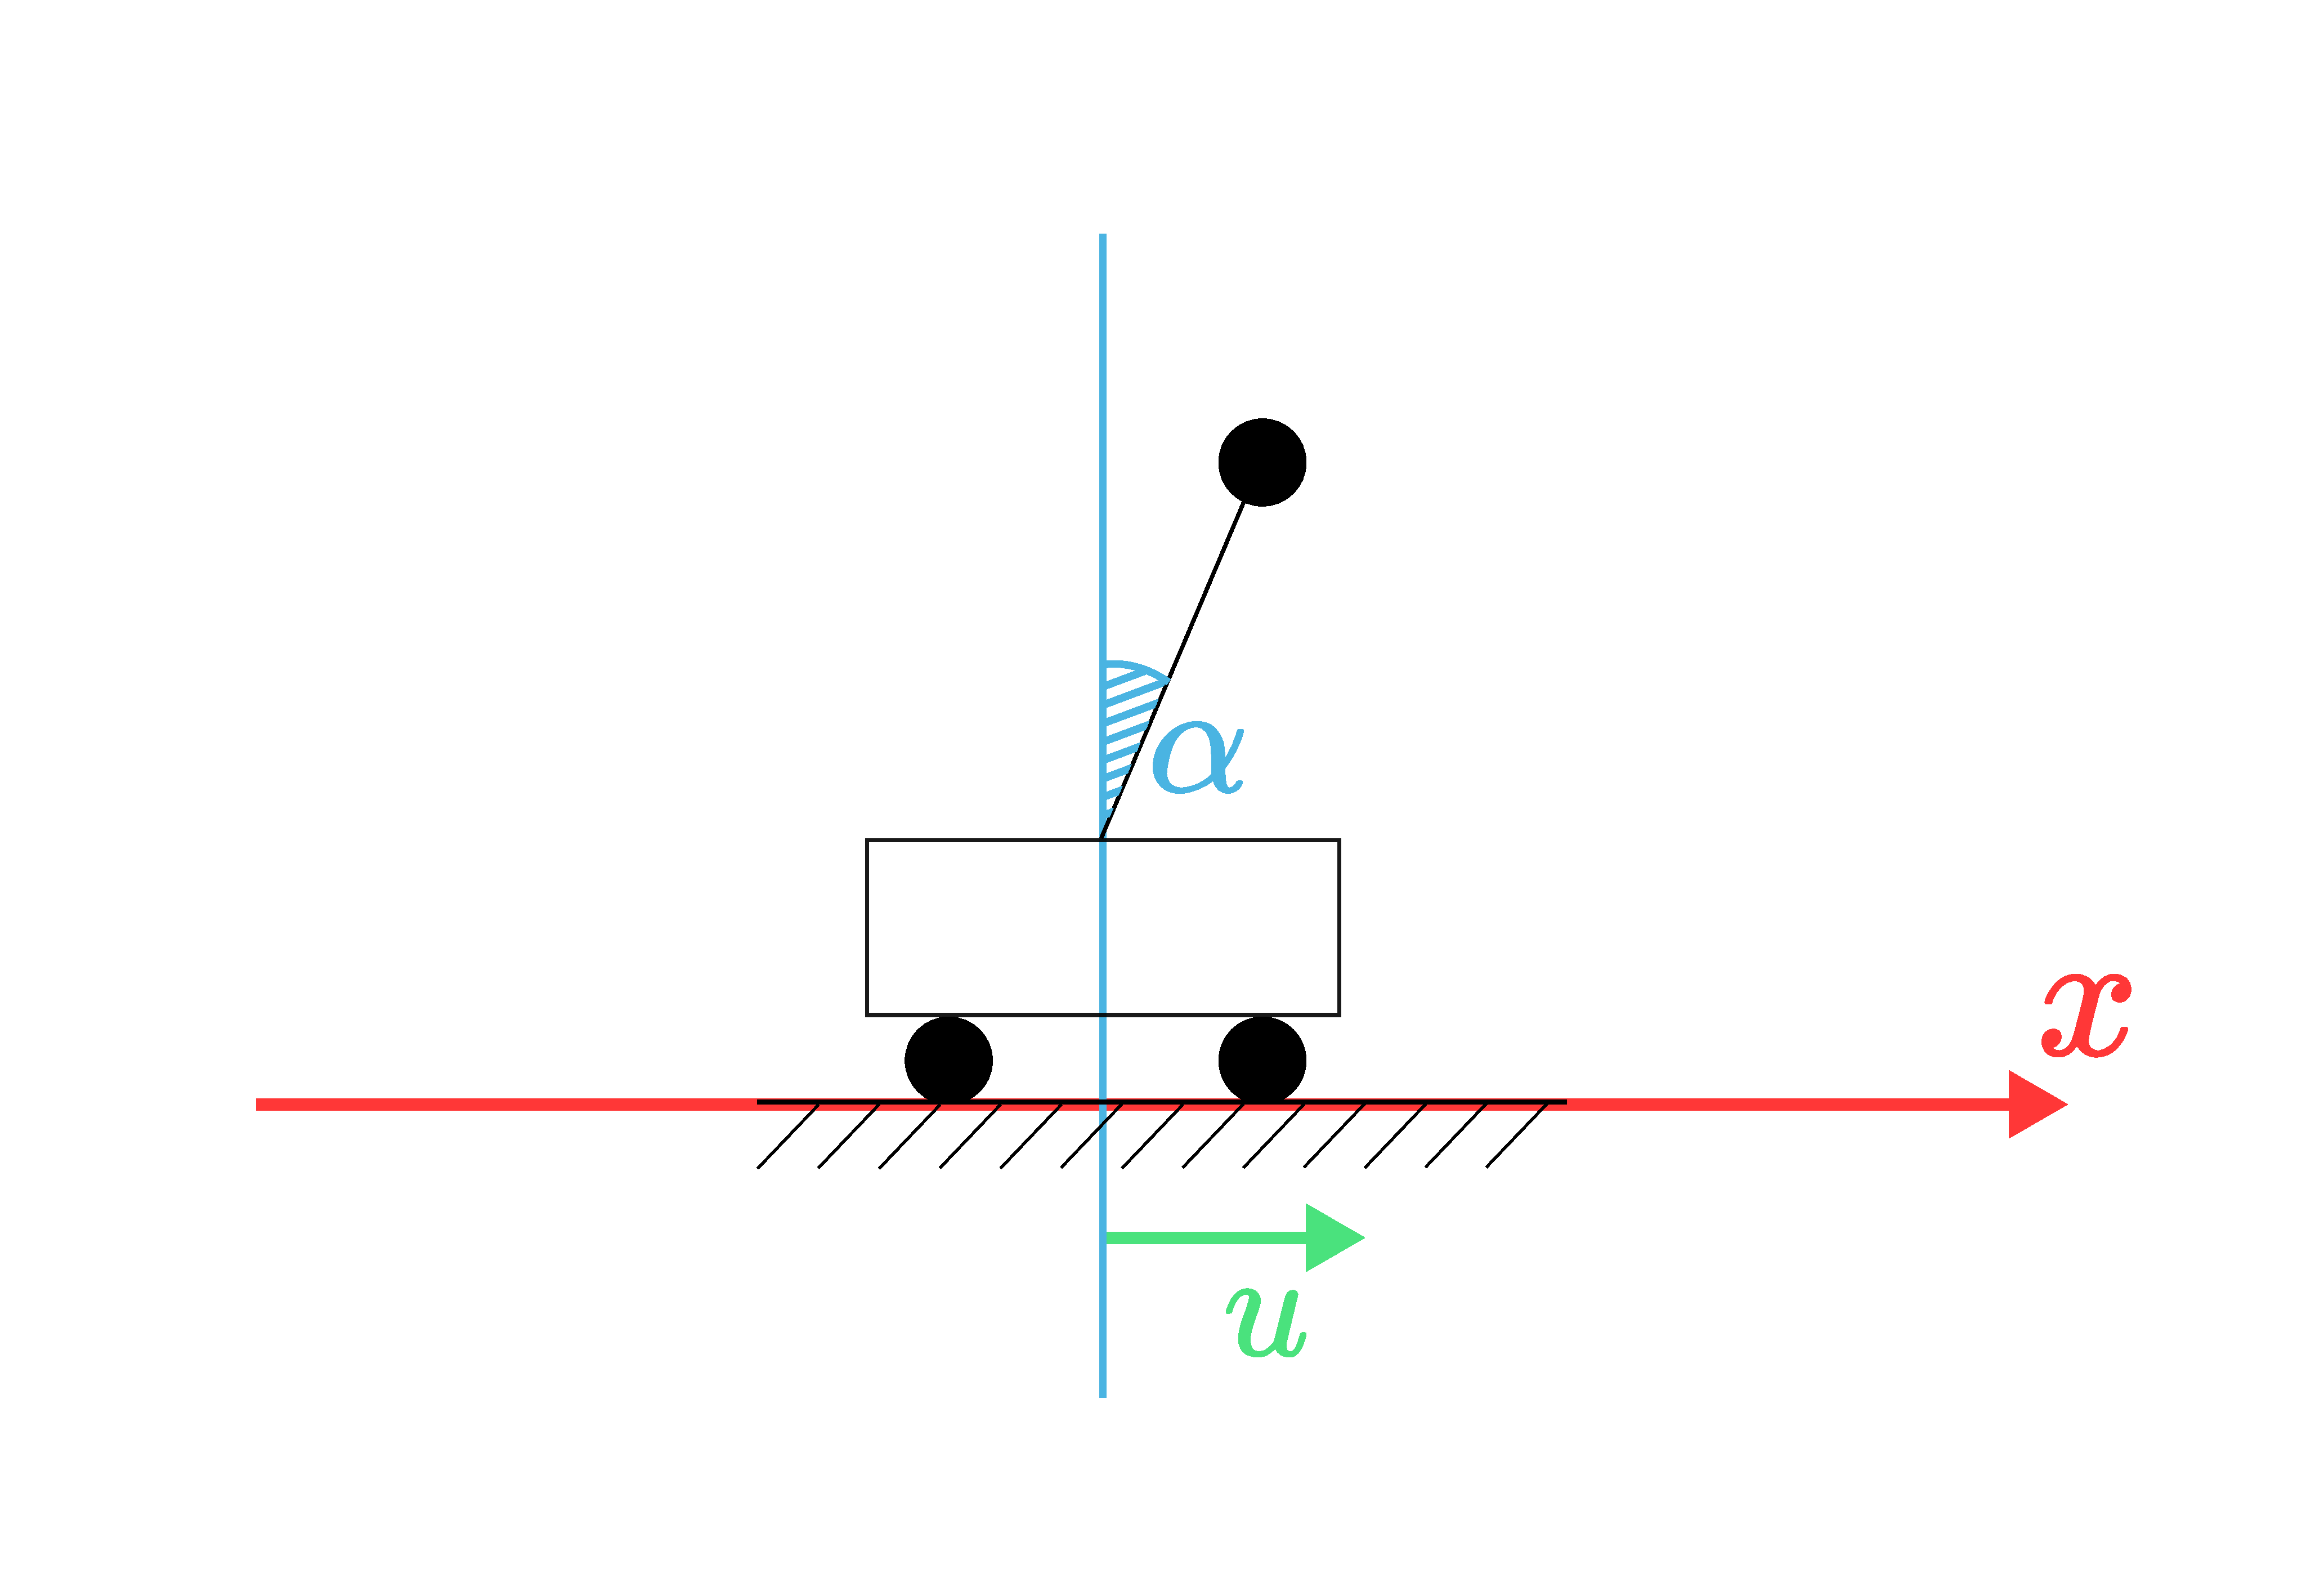
\includegraphics[width=0.4\textwidth]{figures/cartpole.pdf}
    \caption{The cart-pole system, with both coordinates $x$ and $\alpha$, as well as the control variable $u$ (a linear force on the cart) clearly labeled.}
\end{figure}

We focused our experiments on \textit{LTC} cells with various neuron counts as an investigation. For all of our cart-pole experiments we use the following reward: 

\begin{align*}
    r_t = 
    \begin{cases}
        -2 & \text{if} ~|\alpha|>\alpha_\text{max} ~\text{(failure)}\\
        1-q u^2 & \text{otherwise} 
    \end{cases}
\end{align*}

Where $q=0.2$ is a penalty on control (where $u$ is a force measured in newtons) and where the angle $\alpha_\text{max}=0.209$ is used to define failure (with $\alpha$ the pole-angle measured in radiant).  \\

\begin{figure}[h!]
    \centering
    \includegraphics[width=0.4\textwidth]{figures/5n_solution.pdf}
    \caption{Visualization of (from the top down) observation, action and neuron activations together for a $5$ neuron LTC cell trained with PPO on a cart-pole \textit{Mujoco} environment. The activation plot is structured as follows, each row correspond to a single neuron is colored along the $t$ horizontal axis according to the activation $x_i$ of that neuron at time $t$.}
\end{figure}

We find that the LTC cell trained with PPO can find efficient solutions to the cart-pole problem, but that it does so with a particularly low sample efficiency (compared to a reference \textit{MLP} model trained with a perceptron). 




\subsection{Neuron Count Experiments}
We run experiments with various neuron counts ($5,6,7,8,16,$ and $32$ neurons). The main questions we aim to answer with such a protocol are "\textit{Is there a minimum neuron count to solve such a problem?}" (and how different is it from the minimum neuron count with a perceptron) and "\textit{how does the neuron count affect the quality of solution?}". 


\subsection{Sample efficiency}
\textbf{TODO : Influence of nc and mask?}
\begin{figure}[h!]
    \centering
    \includegraphics[width=0.45\textwidth]{figures/convergence_rate.png}
    \caption{}
\end{figure}

\subsection{Resilience to noise?}
\textbf{TODO : Influence of nc and mask?}

\subsection{Resilience to noise?}
\textbf{TODO : Influence of nc and mask?}

\subsection{Discussion of the results}
\textbf{TODO : Discuss the usability of the learned policies, what can we infer from this}


\subsection{Further work section}
\textbf{TODO : Discuss what I didn't have time to do?}